\documentclass{beamer}

\usepackage{amssymb,amsmath}
\usepackage{graphicx}
\usepackage{url}
\usepackage{color}
\usepackage{pagenote}[continuous,page]
\usepackage{relsize}		% For \smaller
\usepackage{url}			% For \url
\usepackage{epstopdf}	% Included EPS files automatically converted to PDF to include with pdflatex

%For MindMaps
% \usepackage{tikz}%
% \usetikzlibrary{mindmap,trees,arrows}%

%%% Color Definitions %%%%%%%%%%%%%%%%%%%%%%%%%%%%%%%%%%%%%%%%%%%%%%%%%%%%%%%%%
%\definecolor{bordercol}{RGB}{40,40,40}
%\definecolor{headercol1}{RGB}{186,215,230}
%\definecolor{headercol2}{RGB}{80,80,80}
%\definecolor{headerfontcol}{RGB}{0,0,0}
%\definecolor{boxcolor}{RGB}{186,215,230}

%%% Save space in lists. Use this after the opening of the list %%%%%%%%%%%%%%%%
%\newcommand{\compresslist}{
%	\setlength{\itemsep}{1pt}
%	\setlength{\parskip}{0pt}
%	\setlength{\parsep}{0pt}
%}

%\setbeameroption{show notes on top}

% You should run 'pdflatex' TWICE, because of TOC issues.

% Rename this file.  A common temptation for first-time slide makers
% is to name it something like ``my_talk.tex'' or
% ``john_doe_talk.tex'' or even ``discrete_math_seminar_talk.tex''.
% You really won't like any of these titles the second time you give a
% talk.  Try naming your tex file something more descriptive, like
% ``riemann_hypothesis_short_proof_talk.tex''.  Even better (in case
% you recycle 99% of a talk, but still want to change a little, and
% retain copies of each), how about
% ``riemann_hypothesis_short_proof_MIT-Colloquium.2000-01-01.tex''?

\mode<presentation>
{
  \usetheme{CambridgeUS}		% bem bacana - menu superior
  \usecolortheme{default}		% branco, azul clarinho
  \useoutertheme{default}
  \useinnertheme{circles}
  \setbeamercovered{invisible}
}

\beamertemplatenavigationsymbolsempty

%% Better looking blocks
\setbeamercolor{block title alerted}{use=structure,fg=black,bg=red!80!black}
\setbeamercolor{block body alerted}{use=structure,fg=black,bg=white!90!black}

\setbeamercolor{block title}{use=structure,fg=black,bg=blue!60!white}
\setbeamercolor{block body}{use=structure,fg=black,bg=white!90!black}

\usepackage[english]{babel}
\usepackage[latin1]{inputenc}
\usepackage{subfigure}

\usepackage{times}
\usepackage[T1]{fontenc}

%% makes the ppagenote command for figure references at the end.
\makepagenote
\renewcommand{\notenumintext}[1]{}
\newcommand{\ppagenote}[1]{\pagenote[Page \insertframenumber]{#1}}


\usepackage{tikz}
\usetikzlibrary{arrows,shapes}

\title[GB13604]{GB13604 - Maths for Computer Science}
\subtitle[]{Lecture 7 -- Counting Part II}
\author[Claus Aranha]{Claus Aranha\\{\footnotesize caranha@cs.tsukuba.ac.jp}}
\institute[COINS]{College of Information Science}
\date[2018-11-21]{2018-11-21\\{\tiny Last updated \today}}

\tikzstyle{vertex}=[circle,fill=black!25,minimum size=10pt,inner sep=0pt]
\tikzstyle{blue vertex}=[circle,fill=blue!100,minimum size=10pt,inner sep=0pt]
\tikzstyle{red vertex}=[circle,fill=red!100,minimum size=10pt,inner sep=0pt]
\tikzstyle{yellow vertex}=[circle,fill=yellow!100,minimum size=10pt,inner sep=0pt]
\tikzstyle{edge} = [draw,thick,-]
\tikzstyle{pedge} = [draw,thick,.]
\tikzstyle{red edge} = [draw, thick,-,red!50]
\tikzstyle{black edge} = [draw, line width=2pt,-,black!20]
\tikzstyle{weight} = [font=\smaller]

\begin{document}

\begin{frame}
  \maketitle

  \begin{center}
    {\smaller This course is based on Mathematics for Computer Science, Spring
    2015, by Albert Meyer and Adam Chlipala, Massachusetts Institute
    of Technology OpenCourseWare.}
    
    
\includegraphics[width=0.2\textwidth]{../img/by-nc-sa}
  \end{center}
\end{frame}

\section{Introduction}

\begin{frame}
  \frametitle{Week 6 and 7 summary}

  {\larger
    {\bf Counting}

    \bigskip

    \begin{itemize}
    \item \structure{Sums and Products}
    \item \structure{Asymptotics}
    \item \alert{Counting with Bijections}
    \item \alert{Repetitions and Binomial Theorem}
    \item \alert{Pigeonhole Principle}
    \end{itemize}
  }
\end{frame}

\begin{frame}
  \frametitle{Counting Rules}
  
  {\larger

    \structure{How do you count things} and \structure{Why is it important}?

    \begin{itemize}

    \item Count the number of people by counting heads;
    \item Count the number of people by counting \alert{tables};
    \item Count the number of cards in a deck;
    \item Count the number of \structure{possible card combinations};
    \item Count the number of \alert{steps in an algorithm};
    \item count the number of \alert{passwords};
    \item count the number of {\bf \alert{problem configurations}}
      
    \end{itemize}
  }
\end{frame}

\subsection{The Bijection Rule}

\begin{frame}
  \frametitle{The Bijection Rule}

  {\larger

    The {\bf Bijection Rule} states that if there is a bijection $A
    \to B$, then $|A| = |B|$.

    \bigskip

    This means that if there is a \alert{set $A$ that we don't know
      the size}, but we make a bijection to a \structure{set $B$ that
      we know the size}, then we can discover the size of $A$.

    \bigskip

    We will use this rule a lot in this class.
  }
\end{frame}

\begin{frame}
  \frametitle{The Bijection Rule: Example}

  {\larger

    A card game has five colors of cards: \structure{Blue, Green, Red,
      Black and White.}

    \bigskip
    
    How many different decks can you build of \structure{12 cards}?

    \vfill

    \begin{center}
      \begin{tabular}{ccccc}
        000 & (none) & 0000 & 00 & 000\\
        blue & green & red & black & white\\
      \end{tabular}
    \end{center}
  }  
\end{frame}

\begin{frame}
  \frametitle{Bijection Rule: Example}

  {\larger
    \begin{itemize}
    \item {\bf Set $A$}: Number of 12-card deck with 5 colors.
    \item {\bf Set $B$}: Number of 16-bit strings with 4 ``1''.
    \end{itemize}

    \bigskip
    
    \begin{center}
      \begin{tabular}{ccccccccc}
        000 & 1 & & 1 & 0000 & 1 & 00 & 1 & 000\\
        blue & & green & & red & & black & & white\\
      \end{tabular}
    \end{center}

    \bigskip

    If we can count set $B$, we know the size of set $A$.

    \bigskip

    {\bf Strategy:} Get really good at counting a few things, and use
    bijections to count everything else!  }
\end{frame}

\subsection{Counting Sequences}

\begin{frame}
  \frametitle{Counting Sequences}

  {\larger
    
    Our strategy is to create rules for \structure{couting sequences}.

    \bigskip
    
    We define a \structure{sequence} as ``choosing something from set
    A'' then ``choosing something from set B'' then ``choosing
    something from set C'', etc.

    \bigskip

    If we can define rules for counting sequences, and define rules
    for representing other objects as sequences, we can solve many
    complex counting problems!
  }
\end{frame}

\begin{frame}
  \frametitle{Starting from the basics: Sum rule and product rule}

  {\larger

    {\bf The Sum Rule:} If Two sets (A,B) are disjoint, the size of
    the set that combines $A$ and $B$ is:
    \begin{equation}
      |A \cup B| = |A| + |B|
    \end{equation}

    \bigskip

    {\bf The Product Rule:} If $|A| = m$ and $|B| = n$. The size of
    the sequence of choosing one thing from $A$ and one thing from $B$
    is:
    \begin{equation}
      |A \times B| = |A| \times |B|
    \end{equation}
    
  }
\end{frame}

\begin{frame}
  \frametitle{Sum Rule/Product Rule Example}

  {\larger
    
    You have \structure{3 blue shirts}, \alert{5 black shirts},
    \structure{4 pants} and \alert{3 skirts}.  If you wear one top and one
    bottom, {\bf how amany different cloth sets do you have}?

    \vfill
    
    \begin{itemize}
    \item {\bf TOP}: $|A| = |\text{Blu} \cup \text{Bla}| = 3 + 5 = 8$
    \item {\bf BOTTOM}: $|B| = |P \cup S| = 4 + 3 = 7$
    \item {\bf TxB Set}: $|A \times B| = 7 \times 8 = 56$
    \end{itemize}

    \bigskip

    You have 56 combinations of tops and bottoms.
  }
\end{frame}

\begin{frame}
  \frametitle{Product Rule and Bit Strings}

  {\larger

    How many bit strings exist of size \structure{n}?

    \bigskip

    We can think of this problem as a \alert{sequence of choices}:
    \begin{itemize}
    \item We choose 1st bit from $\{0,1\}$
    \item We choose 2nd bit from $\{0,1\}$
    \item $\ldots$
    \item We choose nth bit from $\{0,1\}$
    \end{itemize}
    
    \begin{equation}
      \{0,1\}^n ::=
      \{0,1\}\times\{0,1\}\times\{0,1\}\times\ldots\times\{0,1\}
    \end{equation}
    So by the product rule:
    \begin{equation}
      |\{0,1\}^n| = |\{0,1\}|^n = 2^n
    \end{equation}
  }
\end{frame}

\subsection{Counting Passwords}

\begin{frame}
  \frametitle{Password Counting}
  
  {\larger

    How many different passwords exist with these rules?

    \bigskip

    \begin{itemize}
    \item Digits and letters are acceptable;
    \item From 6 to 8 characters;
    \item Starts with a letter;
    \item Case sensitive;
    \end{itemize}
  }
\end{frame}

\begin{frame}
  \frametitle{Password Counting}

  {\larger 
    \begin{itemize}
    \item $L ::= \{a,b,c,\ldots,y,z,A,B,C,\ldots,Y,Z\}, |L| = 52$
    \item $D ::= \{0,1,2,3,4,5,6,7,8,9\}, |D| = 10$
    \item $P_n ::=$ Passwords with $n$ characters.
    \item $P_n ::= L \times (L\cup D)^{n-1}$

      \bigskip

    \item We want to know: $P_6 \cup P_7 \cup P_8$
    \end{itemize}
  }
\end{frame}

\begin{frame}
  \frametitle{Password Counting}

  {\larger

    \begin{itemize}
    \item Size of the password space: $|L\times(L\cup D)^5 \cup
      L\times(L\cup D)^6 \cup L\times(L\cup D)^7|$

      \bigskip
      
    \item Sum Rule:\\
      $|L\times(L + D)^5| + |L\times(L + D)^6| +  |L\times(L + D)^7|$

      \bigskip
      
    \item Product Rule:\\
      $|L|\cdot(|L| + |D|)^5 + |L|\cdot(|L| + |D|)^6 +  |L|\cdot(|L| + |D|)^7$

      \bigskip
      
    \item Replacing sizes:\\
      $52\times62^5+52\times62^6+52\times62^7$ \\
      \hfill$= 1.8\times10^{14}$ different passwords.
    \end{itemize}

  }
\end{frame}

\subsection{Another Example}

\begin{frame}
  \frametitle{Counting Sevens}

  {\larger
    How many numbers with 4 digits have {\bf at least one 7}?

    \bigskip

    \begin{onlyenv}<2>
    Count cases based on \structure{first occurence of seven}

    \bigskip

    \structure{o}: digit \structure{with} 7 (10 choices) \hfill \alert{x}:
    digit $\neq$ 7 (9 choices)

    \bigskip

    So we define four possible sequences:\\
    7\structure{ooo}\hfill\alert{x}7\structure{oo}\hfill\alert{xx}7\structure{o}\hfill\alert{xxx}7

$10^3$ \hfill $9\cdot10^2$ \hfill $9^2\cdot10$\hfill $9^3$
    
    \bigskip

    \begin{center}
      3439
    \end{center}
    \end{onlyenv}
  }
\end{frame}

\section{Generalized Rules}

\begin{frame}
  \frametitle{Generalized Product Rule}

  {\larger

    How can I choose a \alert{group of 5 students} from a class of 25?

    \bigskip

    {\bf Thinking with a sequence of choices:}
    \begin{itemize}
    \item Select 1 student from 25
    \item Select 1 student from 24
    \item Select 1 student from 23
    \item Select 1 student from 22
    \item Select 1 student from 21
    \end{itemize}
    
    \bigskip
    
    $|G| = 25\cdot24\cdot23\cdot22\cdot21$
  }
\end{frame}

\begin{frame}
  \frametitle{Generalized Product Rule}

  {\larger

    If we have to choose $k$ elements from a set of size $n$,
    \alert{without repetition}:

    \begin{equation}
      n\cdot n-1\cdot\ldots\cdot n-k \text{ OR } \frac{n!}{(n-k)!}
    \end{equation}

  }

  
\end{frame}

\begin{frame}
  \frametitle{Generalized Product Rule: Chess Example}

  {\larger
  How many different ways can we put \structure{a bishop, a knight and
    a pawn} in a chessboard \alert{in different rows and columns}?

  \bigskip

  \begin{center}
    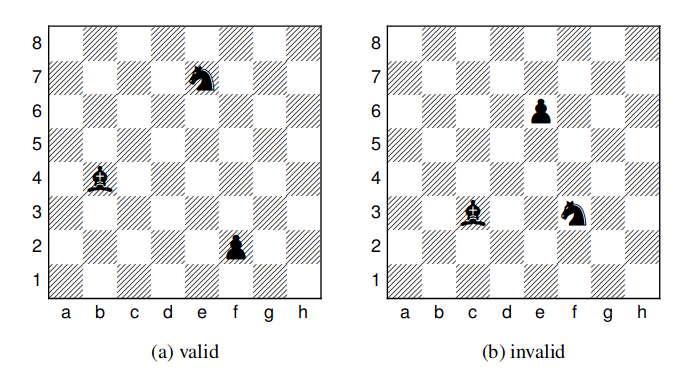
\includegraphics[width=0.8\textwidth]{../img/chess_count1}
  \end{center}
  }
  
\end{frame}

\begin{frame}
  \frametitle{Generalized Product Rule: Chess Example}

  {\larger
  Let's represent this problem as a \structure{Sequence of Choices}:
  \begin{itemize}
  \item Column for Knight: $c_n$ (from 8)
  \item Column for Bishop: $c_b$ (from 7)
  \item Column for Pawn: $c_p$ (from 6)
  \item Row for Knight: $r_n$ (from 8)
  \item Row for Bishop: $r_b$ (from 7)
  \item Row for Pawn: $r_p$ (from 6)
  \end{itemize}

  \bigskip

  Total Positions: $c_nc_bc_pr_nr_br_p = 8\cdot7\cdot6\cdot8\cdot7\cdot6$
  }
\end{frame}

\subsection{The Division Rule}

\begin{frame}
  \frametitle{The Division Rule}

  {\larger
    
  I could count the number of students in this room by \alert{counting
    the number of {\bf hands} in the room}.

  \bigskip

  \begin{itemize}
  \item $A$ - number of students in the room
  \item $B$ - number of hands in the room    
  \end{itemize}

  Since every student \structure{maps} to two hands, then:

  \begin{equation}
    |B| = 2|A|
  \end{equation}

  \vfill

  The \structure{Division Rule} says that if there is a \alert{k-to-1}
  relationship between $A$ and $B$, then $|B| = k|A|$.

  }
\end{frame}

\begin{frame}
  \frametitle{Chess Example 2}

  {\larger How many different ways can we put \structure{two towers}
    in a chessboard \alert{in different rows and columns}?

  \bigskip

  \begin{center}
    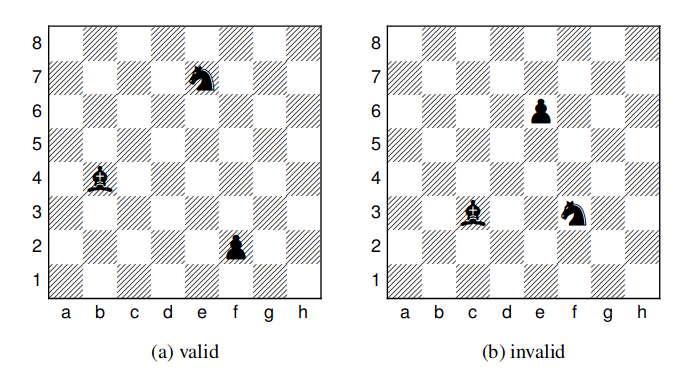
\includegraphics[width=0.8\textwidth]{../img/chess_count1}
  \end{center}
  }
  
\end{frame}

\begin{frame}
  \frametitle{Chess Example 2}

  {\larger
  Let's represent this problem as a \structure{Sequence of Choices}:
  \begin{itemize}
  \item Column for Tower 1: $c_1$ (from 8)
  \item Column for Tower 2: $c_2$ (from 7)
  \item Row for Tower 1: $r_1$ (from 8)
  \item Row for Tower 2: $r_2$ (from 7)
  \end{itemize}

  \bigskip

  Total Positions: $c_1c_2r_1r_2 = (8\cdot7)^2$ \hfill \alert{WRONG!}
  }
\end{frame}

\begin{frame}
  \frametitle{Chess Example 2}

  {\larger
    Total Positions: $c_1c_2r_1r_2 = (8\cdot7)^2$ \hfill \alert{WRONG!}

    \bigskip

    (2,7,3,4) is the same as (7,2,4,3) -- \alert{The two towers are equal!}

    \bigskip

    Every position can be ``doubled'' by switching the towers, so we
    have a 2-1 relationship.

    \bigskip
    
    Therefore, the number of positions is $\frac{(8\cdot7)^2}{2}$
  }
\end{frame}

\subsection{Binomial Theorem}
\begin{frame}
  \frametitle{Counting Subsets}

  {\larger
    How many size 4 subsets of 1 to 13 can we make?
    \begin{itemize}
    \item Set $A ::=$ total permutations of 1 to 13
    \item Set $B ::=$ size 4 subsets
    \end{itemize}

    \bigskip

    Map: \structure{$a_1a_2a_3a_4a_5\ldots a_{11}a_{12}a_{13} \in A$}\\
    To: \alert{$\{a_1a_2a_3a_4\} \in B$}

  }
\end{frame}

\begin{frame}
  \frametitle{Counting Subsets}

  {\larger
    Map: \structure{$a_1a_2a_3a_4a_5\ldots a_{11}a_{12}a_{13} \in A$}\\
    To: \alert{$\{a_1a_2a_3a_4\} \in B$}

    \bigskip
    
    \begin{itemize}
    \item \structure{$a_1a_3a_4a_2$}$a_5\ldots a_{11}a_{12}a_{13}$ also maps.
    \item \structure{$a_1a_2a_3a_4$}$a_{12}\ldots a_{7}a_{9}a_{5}$ also maps.
    \end{itemize}

    \bigskip
    
    For \alert{one subset in $B$}, we can map $4!$
    \structure{permutations of the first four elements, and $9!$
      permutations of the others}.

    \vfill
    
    So the relation between $B$ and $A$ is $4!\cdot9!$-to-1!
    
  }
\end{frame}

\begin{frame}
  \frametitle{Counting Subsets: Binomial Coefficient}

  {\larger
    So to choose a 4 subset out of 13 elements:
    \begin{equation}
      13! = |A| = 9!4!|B|, |B| = \frac{13!}{9!4!}
    \end{equation}

    \vfill

    More generally, to choose $k$ subset from $n$ elements:

    \begin{equation}
      \frac{n!}{n!(n-k)!} = \binom{n}{k}
    \end{equation}

    \hfill ($n$ choose $k$)
  }
\end{frame}

\subsection{2-pair Poker}

\begin{frame}
  \frametitle{Everything Together: 2-pair poker hand}

  {\larger

    In the game of \structure{Poker}, you draw {\bf 5 cards} of a
    52-card deck with \structure{13 ranks} and \structure{4 suits}.

    \bigskip

    \begin{center}
      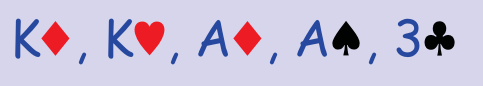
\includegraphics[width=0.6\textwidth]{../img/poker1}
    \end{center}
    
    A \structure{2 pair} hand has
    \begin{itemize}
    \item 2 cards of one rank;
    \item 2 cards of another rank;
    \item 1 card of a third rank;
    \end{itemize}
  }
\end{frame}

\begin{frame}
  \frametitle{2-pair poker hand}

  {\larger
    What is the probability of a 2-pair hand?

    \bigskip
    
    {\bf Total number of hands:} $\binom{52}{5}$

    \bigskip
    
    {\bf Total number of 2-pair:}
    \begin{itemize}
    \item Select first rank (1 of 13)
    \item Select first suits (2 of 4)
    \item Select second rank (1 of 12)
    \item Select second suits (2 of 4)
    \item Select third rank (1 of 11)
    \item Select third suit (1 of 4)
    \end{itemize}
  }
\end{frame}

\begin{frame}
  \frametitle{2-pair Poker Hand}

  {\larger
    1st Rank - 1st Suit - 2nd Rank - 2nd Suit - 3rd rank - 3rd suit\\

    \begin{equation*}
      13\cdot12\cdot11\cdot\binom{4}{2}\cdot\binom{4}{2}\cdot4
    \end{equation*}

    \begin{center}
      \alert{Problem!}

      \includegraphics<2>[width=0.7\textwidth]{../img/poker2}
    \end{center}
  }
\end{frame}

\begin{frame}
  \frametitle{2-pair poker hand -- Problem}

  {\larger
    {\bf Total number of 2-pair:}
    \begin{itemize}
    \item Select \alert{first rank} (1 of 13)
    \item Select first suits (2 of 4)
    \item Select \alert{second rank} (1 of 12)
    \item Select second suits (2 of 4)
    \item Select third rank (1 of 11)
    \item Select third suit (1 of 4)
    \end{itemize}

    \bigskip

    First and Second rank may be switched: \alert{2-to-1} relationship!    
  }
\end{frame}

\begin{frame}
  \frametitle{2-pair Poker Hand -- Fixed!}


  
  {\larger
    1st Rank - 1st Suit - 2nd Rank - 2nd Suit - 3rd rank - 3rd suit\\

    \bigskip
    
    2 Sequences to 1 hand: 2-to-1 relationship: $|A| = 2|B|$

    \bigskip
    
    \begin{equation*}
      \frac{1}{2}\cdot13\cdot12\cdot11\cdot\binom{4}{2}\cdot\binom{4}{2}\cdot4
    \end{equation*}

  }
\end{frame}

\section{Bookkeeper Principle}

\begin{frame}
  \frametitle{The BOOKKEEPER Principle}

  {\larger
    How many permutations has the word \alert{BOOKKEEPER}?

    \bigskip

    \begin{itemize}
    \item Total permutations: $bo_1o_2k_1k_2e_1e_2pe_3r = 10!$

      \bigskip
      
    \item But how many mappings do we have?\\
      $po_1k_1e_1ro_2e_2k_2e_3b$ and\\
      $po_2k_2e_2ro_1e_1k_1e_3b$ and many others...

      \bigskip

    \item 2! permutations of $o_1o_2$, 2! of $k_1k_2$ and 3! of $e_1e_2e_3$
    \item 2!2!3!-to-1 mapping of permutations.            
    \end{itemize}

    \bigskip

    Total Permutations:
    \begin{equation*}
      \frac{10!}{2!2!3!}
    \end{equation*}
  }
\end{frame}

\begin{frame}
  \frametitle{Generalized Multinomial Coefficient}

  {\larger

    Permutation of length $n$ word with $n_1$ a's, $n_2$ b's, $n_3$ c's...

    \bigskip
    
    \begin{equation}%      
      \binom{n}{n_1,n_2,n_3,\ldots,n_k} = \frac{n!}{n_1!n_2!n_3!\ldots n_k!}      
    \end{equation}

    \vfill

    What is the number of ways to rearrange the word \alert{SYSTEMS}?

    \begin{equation*}
      \binom{6}{1,1,3,1,1} = \frac{6!}{3!1!1!1!1!} = 6\cdot5\cdot4 
    \end{equation*}
    
  }
\end{frame}

\subsection{Binomial Theorem}
\begin{frame}
  \frametitle{The Binomial Theorem}

  {\larger
  What is the value of $(a+b)^n$?

  \begin{equation}
    (a+b)^n = \sum^n_{k = 0}\binom{n}{k}a^{n-k}b^k
  \end{equation}

  \vfill
  
  The expansion of $(a+b)^n$ is the sum of all permutations of ``n''
  a's, ``n-1'' a's and 1 b's, ``n-2'' a's and ``2'' b's, ... etc.
  }
\end{frame}

\begin{frame}
  \frametitle{The Binomial Theorem: Examples}

  {\larger

  {\bf Example 1}: The coefficient of $a^3b^5$ from $(a+b)^8$ is the
  number of permutations of $a_1a_2a_3b_1b_2b_3b_4b_5 =
  \frac{8!}{3!5!}$

  \bigskip

  {\bf Example 2}: The coefficient of $bn^2a^3$ from $(b+n+a)^6$ is
  the number of permutations of \structure{banana} = $\frac{6!}{1!2!3!}$

  \bigskip

  {\bf Example 3}: The coefficient of
  $x_1^{k_1}x_2^{k_2}x_3^{k_3}\ldots x_n^{k_n}$ from $(x_1 + x_2 +
  \ldots + x_n)^{k_1+k_2+\ldots+k_n}$ is
  \begin{equation}
    \binom{k_1+k_2+\ldots+k_n}{k_1,k_2,\ldots,k_n}
  \end{equation}
  
  }
\end{frame}

\section{Pigeonhole Principle}

\begin{frame}
  \frametitle{The Pigeonhole Principle}

  {\larger

    {\bf Puzzle:} A drawer has \alert{red socks}, \structure{blue
      socks}, and {\bf black socks}. How many socks do you need to
    pick in the dark to be sure that you have \structure{at least one
      matching pair}?

    \vfill

    \begin{block}{The Pigeonhole Principle}
      If there are more pigeons then pigeonholes, there is at least
      one hole with 2 pigeons.
    \end{block}
  }
\end{frame}

\begin{frame}
  \frametitle{Pigeonhole Example: Same number of hairs in Tokyo!}

  {\larger

    {\bf Claim:} There is a group of \alert{at least 40 people} with
    \structure{the exact number of hairs} in Tokyo.

    \bigskip

    \begin{itemize}
    \item The number of hairs in a person is between 0 and 200.000 (Set $B$)
    \item The number of people in Tokyo is 9.000.000 (Set $A$)
    \item By the \structure{Pigeonhole Principle}, there are at least
      $k$ ($|A|= k|B|$) people in the same group.
    \end{itemize}

    \bigskip

    Therefore, there is \alert{at least one group of 40 people} with
    the exact same number of hairs in Tokyo.

    \vfill

    \begin{center}
      Super Useful!
    \end{center}    
  }
\end{frame}

\begin{frame}
  \frametitle{Pigeonhole Principle: Pitfalls}

  {\larger

    {\bf Correct Example:} If you draw 5 cards from a normal deck,
    then \structure{at least 2 cards} have the same suit.

    \bigskip
    
    {\bf Incorrect Example:} If you draw 5 cards from a normal deck
    then \structure{at least 2 cards} have the {\bf Hearts} suit.\\
    \hfill(\alert{WRONG!})\\
    \hfill(Example: Clubs, Clubs, Clubs, Clubs, Clubs)

    \vfill

    The Pigeonhole principle says that {\bf a group} will have size k,
    but it does not say \alert{which group} will have size k.
  }  
\end{frame}

\begin{frame}
  \frametitle{Pigeonhole Principle: Subset Sums}
  \begin{columns}
    \column{0.7\textwidth}
    
    {\larger
      \begin{itemize}
      \item The image to the right has 90 numbers of 25 digits each;
      \item Are there 2 subsets with the exact same sum?
        \bigskip

      \item<2> Maximum sum: $90\times10^{25}$
      \item<2> Maximum subsets: $2^{90} > 1.237 \times 10^{27}$
        \bigskip

      \item<2> By the \structure{pigeonhole principle}, at least two
        subsets have the same sum!
        
      \end{itemize}
    }
    
    \column{0.2\textwidth}
    \hspace{-1.3cm}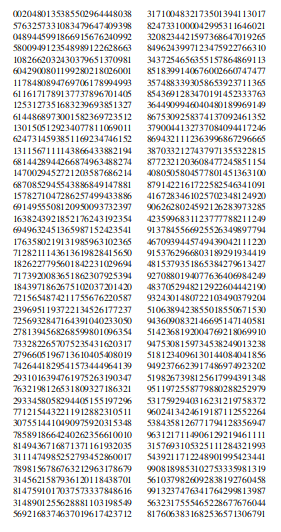
\includegraphics[height=0.8\textheight]{../img/90numbers}
  \end{columns}
\end{frame}

%% TODO: Use Inclusion-Exclusion Principle to prove Euler's Theorem

\section{Conclusion}
\begin{frame}
  \frametitle{Summary}

  \begin{itemize}
  \item How to count permutations
  \item Division Principle: k-to-1 relations
  \item Binomial Theorem
  \item Pigeonhole Principle
  \end{itemize}
\end{frame}


\end{document}
